\documentclass[main]{subfiles}

\begin{document}
\begin{lect} {2019-09-04}
		\section{Метрические пространства}
		\[M \text{ - мн-во,} \q d: M \times M \rightarrow [0; +\infty) \text{ - метрика}\]
		\begin{definition}{Аксиомы метрики}
				\begin{enumerate}
					\item $d(x, y) \geq 0$
					\item $d(x, y) = 0 \rla x = y$
					\item $d(x, y) = d(y, x)$
					\item $d(x, y) \leq d(x, z) + d(z, y)$
				\end{enumerate}
		\end{definition}

		\begin{examples}
				\begin{enumerate}
						\item $M = \R^n \q x \in M \q x = (x_1, ..., x_n)$
							\[d_{\infty}(x,y) = \max_{1 \leq j \leq n}|x_j - y_j|\]
						\item $M = \R^n,$
							\[d_p(x,y) = \root\scriptstyle \os{\text{\small p}}{\ }\of{\sum{|x_j - y_j|}^n_{j = 1}}\]
							%\sqrt[\text{\large p}]{\sum{|x_j - y_j|}^n_{j = 1}}\]
							\[\text{В частности}\q d_2(x, y) = \sqrt{\sum^n|x_j - y_j|^2}\]
						\item $M = C[0,1] \q f, g \in M$
							\[d(f, g) = \sup_{x \in [0, 1]}|f(x) - g(x)| \]
						\item $M = C[-1, 1]$
							\[d(f, g) = \int_{-1}^1 |f-g|\]
				\end{enumerate}
		\end{examples}

		\begin{Utv}
				\[\max_{1 \leq j \leq n}|x_j - y_j| \leq \sqrt{\sum^n_{j = 1}{|x_j - y_j|^2}}
				\leq n \cdot \max_{1 \leq j \leq n} |x_j - y_j|\]
				\[d_{\infty}(x, y) \leq d_2(x, y) \leq n \cdot d_{\infty}(x, y)\]
		\end{Utv}

		\begin{Definition}
				\[x^{(m)} \in M\]
				\[\lim_{m \to \infty} x^{(m)} = x \rla d(x^{(m)}, x) \us{m \to \infty}{\to}0\]
		\end{Definition}

		\begin{examples}
				\begin{enumerate}
						\item $M = C[0, 1] \q d(f, g) = \sup_{x \in [0, 1]} |f(x) - g(x)|$
							\[f^{(m)} \us{d}{\to} f \rla f^{(m)} \us{[0, 1]}{\rightrightarrows} f\]
						\item $M = \R^n,\q d_2(x, y) \q x^{(m)} = (x_1^{(m)},  ..., x_n^{(m)})$
							\[x^{(m)} \us{d_2}{\to} x \rla x^{(m)}_j \to x_j \q \forall j = 1,...n\]
				\end{enumerate}
				Т.о. сх-ть по метрике $d_2$ в $\R^n$ равносильна покоординатной сх-ти
		\end{examples}

		\begin{Theorem}[критерий Коши]
				\[(\R^n, d_2) \qq x^{(m)}=(x_1^{(m)},\ ...,\ x_n^{(m)})\]
				\[x^{(m)} \us{m \to \infty}{\to} x \rla \forall \E > 0 \e N: \forall n, k \geq N \]
				\[d_2(x^{(n)}, x^{(k)}) < \E \text{ (упр, доказывается покоординатно)}\]
		\end{Theorem}

    \begin{remark}
			Аналогичная т. верна не для всех метрич. пр-в
		\end{remark}

		\begin{Example}
			\[M = C[-1, 1] \qq d(f, g) = \int\limits_{-1}^1 |f-g|\]
			\begin{figure}[H]
			    \center{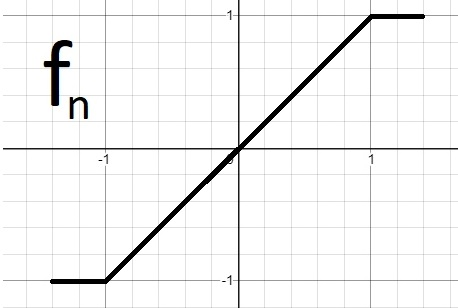
\includegraphics[width=4cm]{pics/1_1}}
			\end{figure}

			\[\{f_n\} \text{ - сх. в себе: }\]
			\[\forall \E > 0\q \e N: \forall n > N,\  p > 0 \q \os{?}{d(f_n, f_{n + p}) < \E}\]
			\[d(f_n, f_{n + p}) = \int_{-1}^1 |f_n - f_{n + p}| = \frac{1}{n} - \frac{1}{n + p} \leq \frac{1}{n} \to 0 \]
			\[\Ra \forall \E \q \e N: \forall n > N,\ p > 0 \q d(f_n, f_{n + p}) < \E\]
			\begin{figure}[h]
				\center{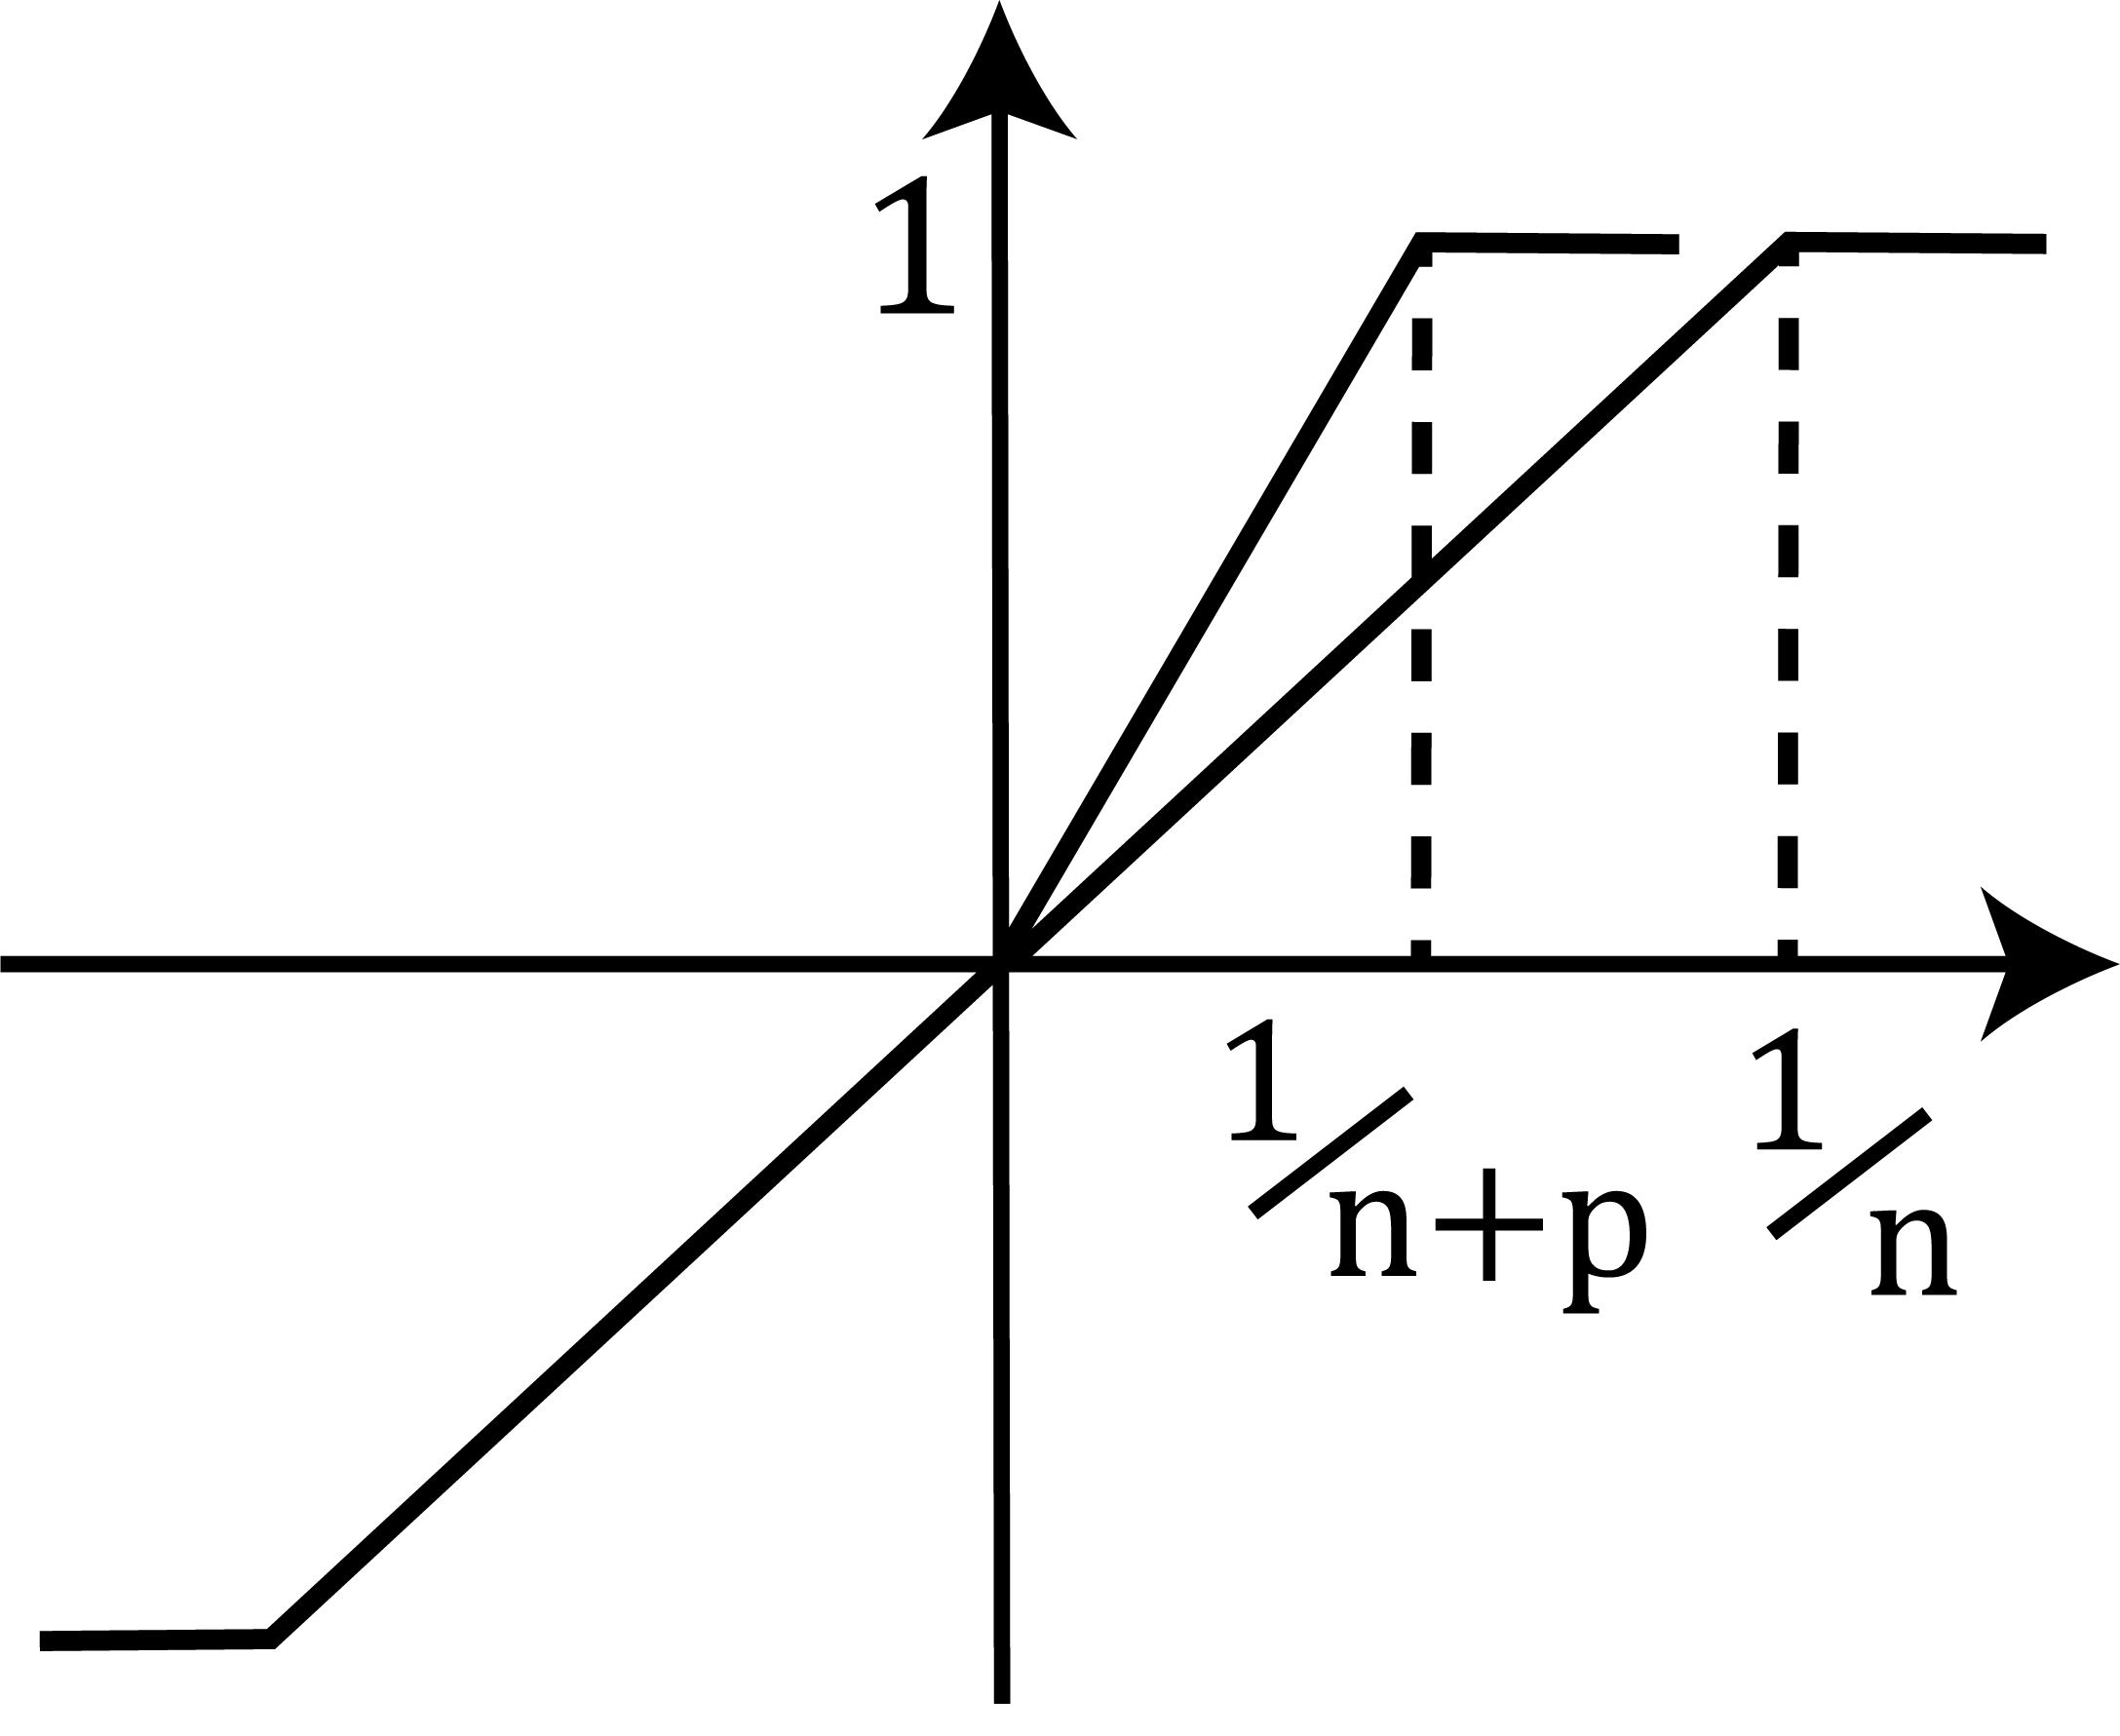
\includegraphics[width=4cm]{pics/1_2}}
			\end{figure}

			Усл. Коши удовл. (сх в себе)
			\[\text{Есть ли } \lim_{n \to \infty} f_n ? \]
			\[g(x) = \sign x \text{ - поточечный предел}\]
			\[\lim_{n \to \infty} \int_{-1}^1 |f_b - g| = 0 \text{, но } g \not \in C[-1, 1]\]
			\[\text{Предположим, что } \e f \in C[-1, 1]: \q \lim{f_n} = f \text{, т.е } \int |f_n - f| \to 0 \]
			\[0 \leq \int_{-1}^1|f-g| \leq \int_{-1}^1 |f_n - f| + \int_{-1}^1 |f_n - g| \us{n \to \infty}{\to} 0 \]
			\[\int_{-1}^1 \us{\q \in C[-1; 1]}{ |f - g|} = 0\]
			\[=\int_{-1}^0 \us{= 0}{|f - g\mid} + \int_{0}^1 \us{= 0}{|f - g|} \Ra
				{\begin{align}
					&f(x) = 1 \q &\forall x > 0\\
					&f(x) = -1 \q &\forall x < 0
				\end{align}}
			\]
			\[\text{ - неустранимый разрыв в точке } x = 0 \RA \lim f_n \text{ не существует} \]
		\end{Example}

		\begin{Upr}
			\[ C[0, 1] \q d(f, g) = \sup_{1 \leq x \leq y} |f(x) - g(x)|\]
			Выполняется ли т. Коши?
		\end{Upr}

		\subsection{Топология в $\R^n$}
		\[d(x,y)=\sqrt{\sum_j^n|x_j-y_j|^2}\]
		\[B(a, r) = \{x \in \R^n : d(a, x) < r\}\]
		\[X \subset \R^n \q X \text{ - откр, если } \forall a \in X \q \e B_a : B_a \subset X\]
		\[X \text{ - замкнуто } \rla X^C \text{ - открыто}\]
		\hsubsubsection{1.1.1}{Топологические св-ва}
		\begin{theorem}[св-ва]
				\begin{enumerate}
						\item $ \displaystyle U_\alpha \text{ - откр. } \forall \alpha \in A \Ra \bigcup_{\alpha \in A} U_\alpha \text{ - откр. }$
						\item $\displaystyle \{U_k\}^N_{k = 1} \text{ - откр. } \Ra \bigcap_{k = 1}^n U_k \text{ - откр}$
						\item $\displaystyle F_\alpha \text{ - замкн. } \forall \alpha \in A \Ra \bigcap_{\alpha \in A}F_\alpha$
						\item $\displaystyle F_k \text{ - замкн. } \Ra \bigcup_{k = 1}^N F_k \text{ - замкн.}$
				\end{enumerate}
		\end{theorem}

		\begin{definition}
				Окрестность т. а:
				\[U\text{ - откр}: a \in U\]
				$\delta	$-окр. т. a:
				\[U_a(\delta) = B(a, \delta)\]
				Прокол. $\delta $-окр. т. а:
				\[\doted{U_a}(\delta) = B(a, \delta) \setminus \{a\}\]
				Внутренность $X \subset \R^n$:
				\[\mathint(X) = \{a \in X: \e B_a \subset X\}\]
				Внешность $X \subset \R^n$:
				\[\ext(X) = \mathint(X^c) = \{b \in X^c : \e B_b \subset X^c\}\]
				Замыкание:
				\[\Cl(X) = (\ext(X))^c\]
				Граница:
				\[\partial X = \Cl(x) \setminus \mathint(X) = \R^n \setminus (\mathint X \cup\ext X)\]
		\end{definition}

		\begin{Examples}
				\[X = B(0, 1)\]
				\[\mathint X = B(0, 1)\]
				\[\ext X = \{x : d(0, x) > 1\}\]
				\[\Cl X = \overline{B}(0, 1) = \{x : d(0, x) \leq 1\}\]
				%Рисунок шарика
				\[\partial X = S(0, 1) = \{x : d(0, x) = 1\}\]
		\end{Examples}

		\begin{upr}
		    Доказать или опровергнуть
				\begin{enumerate}
						\item $\mathint(\mathint X) = \mathint X$
						\item $\partial(\partial X) = \partial X$
						\item $\Cl(\Cl X) = \Cl X$
				\end{enumerate}
    \end{upr}

		\begin{Utv}
				\[X \text{ - замкн } \rla Cl X = X\]
		\end{Utv}

		\begin{Proof}
				\[U \text{ - откр } \q \mathint U = U\]
				\[\Ra X \text{ - замкн } \rla X^c \text{ - откр.} \rla\ext X = \mathint(X^c) = X^c \rla  \]
				\[\Cl X = (\ext X)^c = X^{cc} = X\]
		\end{Proof}

		\begin{definition}
				Ограниченность:
				\[X \subset \R^n,\q \diam X = \sup_{x, y \in X} d(x, y)\]
				\[X \text{ - огр. если } \diam X < \infty \rla \e R > 0: X \subset B(0, R) \text{ (УПР)}\]
		\end{definition}

		\hsubsubsection{1.1.2}{Принцип выбора Больцано-Вейерштрасса}
		\begin{Theorem}[принцип выбора Больцано-Вейерштр.]
				\[\forall \text{ огр. послед. } \{X^{(m)}\} \subset \R^n
					\text{ можно выделить сх. подпослед.}\]
		\end{Theorem}

		\subsection{Компатные множества в $\R^n$}

		\begin{Definition}
				\[K \subset \R^n \text{ - компактное мн-во } \rla \forall
				\text{ откр. покр. можно выд. конеч. подпокр.}\]
				\[\text{Т.е. если } U_\alpha - \text{ откр. }\]
				\[\RA\forall \alpha \in A : K \subset \bigcup_{\alpha \in A}U_\alpha \Ra \e \alpha_1, ..., \alpha_n \in A: K \subset \bigcup^N_{k = 1}U_\alpha\]
		\end{Definition}

		\begin{examples}
				\begin{enumerate}
						\item $[a, b] \subset \R \text{ - компакт.}$
						\item $\displaystyle I := \prod_{j = 1}^n [a_j, b_j] \subset \R^n$
							\begin{figure}[h]
							    \center{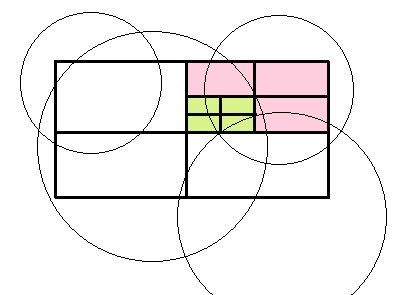
\includegraphics[width=5cm]{pics/1_3}}
							\end{figure}

							\[I_0 \supset I_1 \supset I_2 \supset ... \supset I_n\]
							\[\diam I_n = \frac{\diam I}{2^n} \to 0\]
							\[I_n \text{ - замк}\]
					    \[I_k = \prod_{j = 1} ^n [a_j^{(k)}, b_j^{(k)} ]  \qq \bigcap_{k \in \N} [a_j^{(k)}, b_j^{(k)}] = \{c_j\}\q \forall j \]
							\[[a_j^{(k)}, b_j^{(k)}] \supset [a_j^{(k+1)}, b_j^{(k+1)}] \supset ...\]
							\[\begin{matrix}
								x^* \in \bigcap_{k \in \N} I_k\\
								y^* \in \bigcap_{k \in \N} I_k
							\end{matrix} \RA d(x^*, y^*) \leq \diam I_k \to 0\]
							\[\Ra d(x^*, y^*) = 0 \RA x^* = y^*\]
							\[x^* = \bigcap_{k = 1}^{\infty} I_k\]
							\[x^* \in I \subset \bigcup_{\alpha \in A} U_\alpha \RA \e \alpha^* : x^* \in U_{\alpha^*} \text{ - откр}\]
							\[\e B(x^*, \delta) \subset U_{\alpha^*}\]
							\[\Ra \e N \in \N : I_N \subset U_{\alpha^*}\]
				\end{enumerate}
		\end{examples}
\end{lect}
\end{document}
